\documentclass[conference]{IEEEtran}
\usepackage{amsmath,amssymb,amsfonts}
\usepackage{algorithmic}
\usepackage{graphicx}
\usepackage{textcomp}
\usepackage{xcolor}

\usepackage[numbers]{natbib}
\usepackage{hyperref}
\usepackage{url}
\def\BibTeX{{\rm B\kern-.05em{\sc i\kern-.025em b}\kern-.08em
    T\kern-.1667em\lower.7ex\hbox{E}\kern-.125emX}}
\bibliographystyle{ieeetr}


\begin{document}
\title{A Survey on Hardware Accelerators for Neural Networks}
\author{
\IEEEauthorblockN{Pierre Brosemer}
\IEEEauthorblockA{uitxj@student.kit.edu}
}

\maketitle

\begin{abstract}
This will be my Abstract in \LaTeX.
I am going to write this when I have almost finished the essay since it will probably be easier to give an overview over the topic once the full paper is finished.
The availability of efficient hardware was one of the key factors, which lead to the rise of Neural Network \cite{historyfpgas}. 
\\
\end{abstract}

\section{Introduction}
Artifical Neural Networks (more often Neural Networks) are one of the most promising technologies in the current era of computer science. Neural Networks can be deployed in an enourmous variety of categories and have shown major improvements in these categories, most prominently in Speech and Image Recognition \cite{speech_recognition1} that exceeded prior methods. The field of Artifical Intelligence covers a wide variety of concepts. This paper will mainly cover the subcategory of Deep Learning, more specifically Neural Networks, which falls under the category of Machine Learning. 
\\
Neural Networks are at it's core a very broad simplification of the biological brain consisting of many interconnected neurons, called nodes in Neural Networks. The nodes in a Neural Network are  arranged in different layers. Each node passes on a weighted function to a node in the next layer. If this value is above a certain threshhold the node will be activated. By changing the weights of each node a learning process similiar to that of their biological counterpart is simulated \cite{nn_basics}.
\begin{figure}[h]
	\caption{Typical representation of a Neural Network}
	\centering
	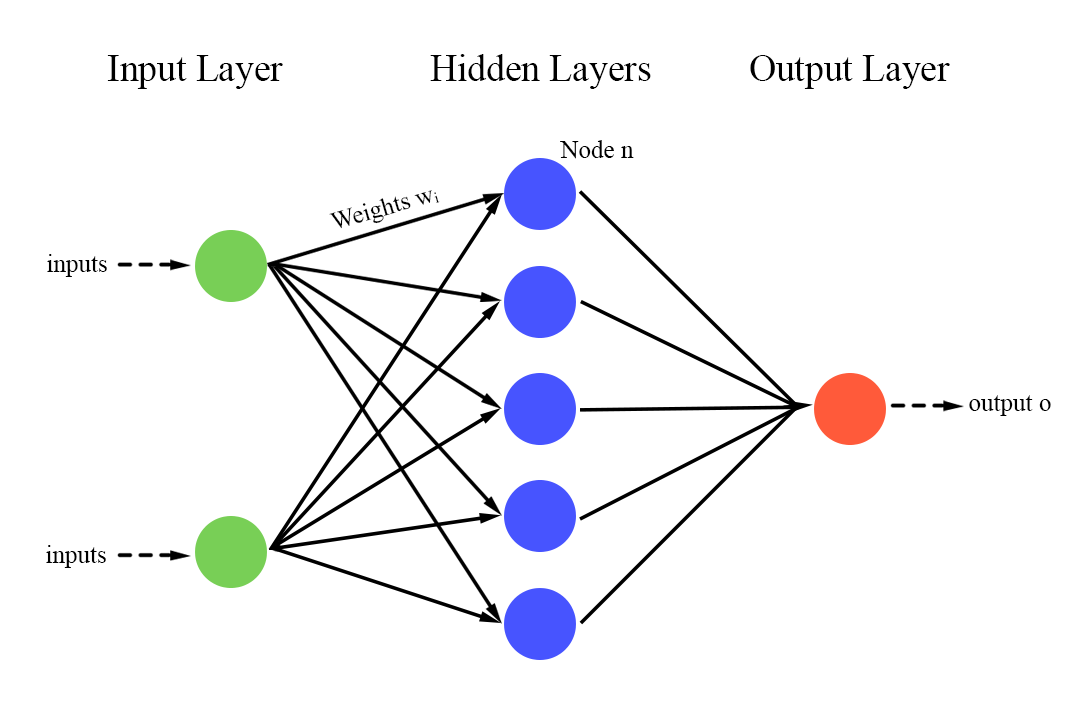
\includegraphics[width=\linewidth]{pictures/neuralnetwork.png}
\end{figure}

The development of a Neural Network consists of two different stages. Firstly a training phase where the Neural Network gets an input and compares the resulting output (prediction) with that of a real-world dataset. The error can then be incorparated into the network by changing the different weights, also called backpropagation. Secondly an inference phase, where the network get's an input and makes a prediction. The Neural Network has a larger computational effort in the training phase as more data is processed, aswell as the weights needing calibration.
\\
\\
With some Neural Networks having over 150 layers \cite{densely_network} up to billions of Multiplications can take place in a single Neural Network. The vast amount of computational power needed for training and using neural network lead to the need for specialised hardware, which contributed much to the success seen in modern day implementations. The research on hardware is still ongoing and is one of the most important topics in achieving better and faster results for Neural Networks. As a result of the timeliness of the topic this survey will only cover a status quo of the current Hardware.
\\

\section{Different Types of Hardware}
Most of Computations needed for inference and training include Matrix-Vector Products, caused by the input data being run through the network.
Furthermore  the dimension of the input data plays a key role in the amount of computation needed. Lets say a single image has 1000 pixels resulting in 1000 different data points that the Neural Network has to compute. To efficiently compute the vast amount of data fast memory accesses or inplace computations of the values is needed. Since these Calculations need to be done for the number of nodes good parallelization is needed to efficiently run Neural Networks.
\\
Hardware Accelerators for Neural Networks can be divided into 4 main classes: CPUs, GPUs, FPGAs and ASICs. The focus can be placed on the latter 3 since CPUs mostly fall short in terms of computational power for Neural Networks. 
CPUs are needed for a wide variety of tasks requiring a flexible system to execute instructions. As a result a CPU is good at executing serial instructions in parallel, resulting in a good general parallelization.
Both of the points mentioned above, that are needed for the specialised hardware for Neural Networks, are not met for CPUs. They are limited by their small amount of cores hindering the ability to parallelize the same instruction. Moreover a CPU usually works by fetching an instruction and executing it making the training and inference phase slow \cite{capra2020updated}. While working on Neural Networks CPUs are accompanied by Underutilization, achieving factors of less than 1/10 of that other alternatives \cite{nurvitadhi2016accelerating}. Nonetheless Intel is working on accelerating CPUs producing librarys for their Intel Xeon Processor \cite{intelnn}.
\\
Another point to consider is the different requirements needed for both the training and inference phase. During the inference phase certain approximasations can be made to achieve faster results, which can't be made for the training phase. This derives in some Hardware only being designed for the inference phase. 

\section{Graphics Processing Unit}
The Graphics Processing Unit (GPU) is a piece of specialised Hardware originally designed for the rendering of images in a Computer. The rendering process requires vast amounts of floating point operations resulting in the GPU having hundreds of cores with many individual caches to store the computation. To add on the GPU has more units dedicated to floating-point operations. This makes the GPU an excellent tool for working with Neural Networks since the their specifications align with those for rendering Graphics. With over thousands cores the GPU can parallelize the matrix multiplications needed for training and achieve fast training times. 
\begin{figure}[h]
	\caption{Differt Layouts comparing CPU and GPU: The GPU has more cores with more individual Caches \cite{intelpic_comparison}}
	\centering
	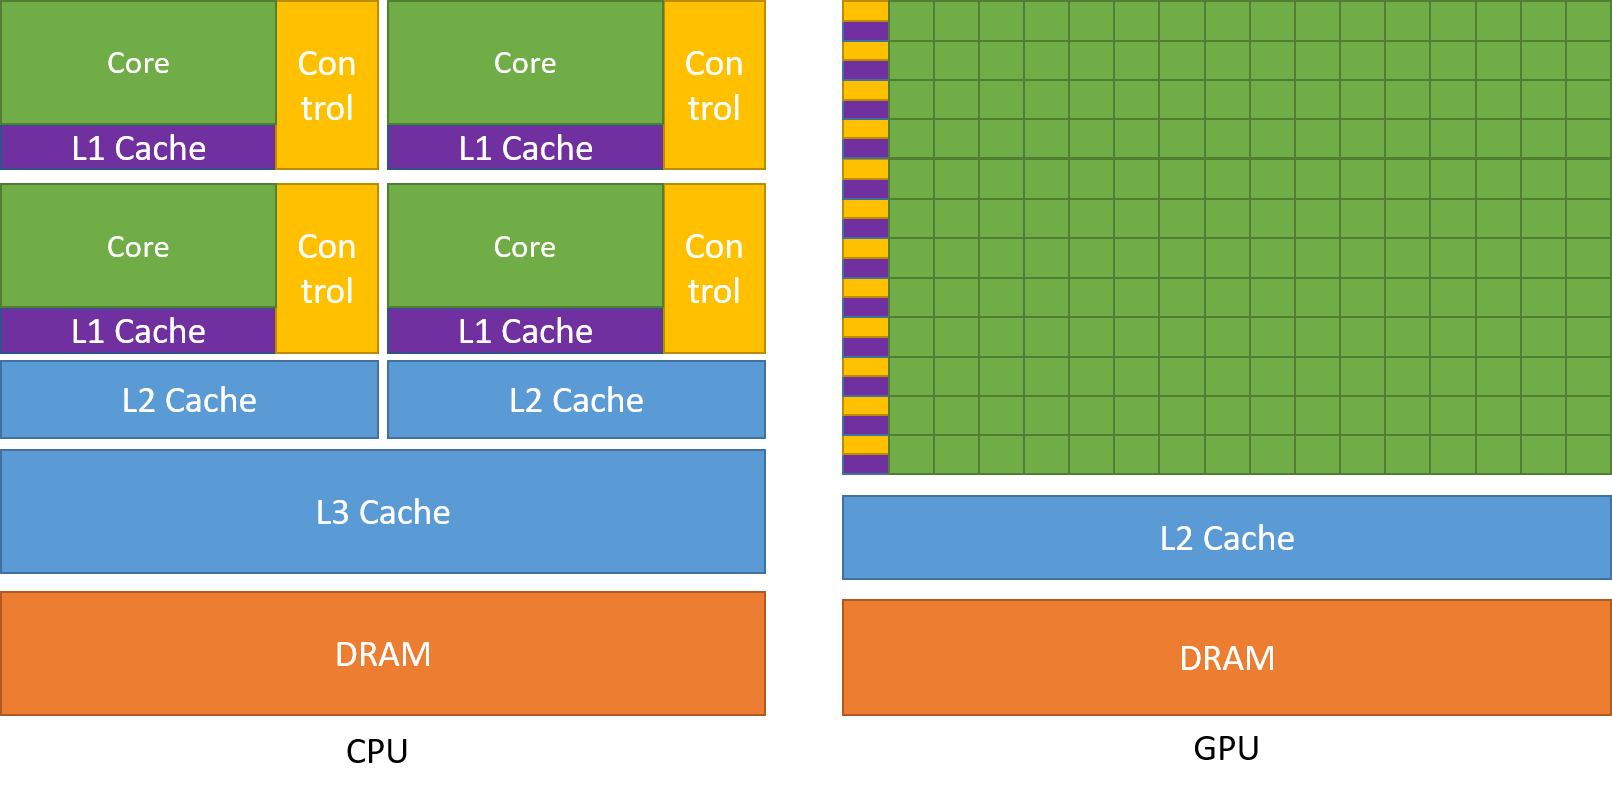
\includegraphics[width=\linewidth]{pictures/intel_comparison.png}
\end{figure}

Through this structure high memory throughput and good Execution of parallel instructions is given. Nvidia ,one of the leaders in manufactoring, is implementing the their specialised Deep Learning Units with normal cores plus additional Tensor cores \cite{nvidiav100}. Tensor Cores essentiely multiply 2 FP-16 Matrix (Floating Point 16 bit) and being able to add a third Matrix all in a single operation, performing 64 operations per clock \cite{tensorcores}. Their newest product the Nvidia A100 uses the third generation of tensor cores with better precision.
Another way GPUs accelerate is by making use of the sparsity of matrices used for calculating the different functions, more on that later.
GPUs can be seen as the most used hardware option for neural networks for general scientific usage \cite{mostusedgpu}. They are mostly used for training, but can also be used for the inference phase because of their flexible hardware structure \cite{capra2020updated}. They are specifically fast in training due to their ability to work through large amounts of data quickly (having a high memory bandwidth).

\section{Field-programmable Gate Array}


\newpage
\quad
\newpage

\bibliography{References}
\end{document}
